\documentclass[paper=a4,fontsize=11pt]{scrartcl} % KOMA-article class



%\usepackage[1-5]{pagesel}
\usepackage[english]{babel}
\usepackage[utf8]{inputenc}
\usepackage[protrusion=true,expansion=true]{microtype}
\usepackage{amsmath,amsfonts,amsthm}     % Math packages
\usepackage{graphicx}                    % Enable pdflatex
\usepackage[svgnames]{xcolor}            % Colors by their 'svgnames'
\usepackage{geometry}
	%\textheight=700px                    % Saving trees ;-)
%\usepackage{url}
\usepackage[colorlinks=true,
linkcolor=darkgray,
urlcolor=darkgray]{hyperref}
\usepackage{float}
\usepackage{etaremune}
\usepackage{wrapfig}
\usepackage{bibentry}
%\nobibliography*
\usepackage{natbib}
%\bibliographystyle{unsrtnat}
\usepackage{attachfile}

\frenchspacing              % Better looking spacings after periods
%%\pagestyle{empty}           % No pagenumbers/headers/footers

%\addtolength{\voffset}{-40pt}
%\addtolength{\textheight}{20pt}

\setlength\topmargin{0pt}
\addtolength\topmargin{-\headheight}
\addtolength\topmargin{-\headsep}
\setlength\oddsidemargin{0pt}
\setlength\textwidth{\paperwidth}
\addtolength\textwidth{-2in}
\setlength\textheight{\paperheight}
%\addtolength\textheight{-3in}
\addtolength\textheight{-2in}
\usepackage{layout}



\usepackage[]{scrlayer-scrpage}  %put headsepline in brackets for horizontal headline
\clearpairofpagestyles
\rofoot{\color{gray}\today}
\cfoot{\pagemark}
%\ihead{Title description}



%%% Custom sectioning}{sectsty package)
%%% ------------------------------------------------------------
\usepackage{sectsty}

\sectionfont{%			            % Change font of \section command
	\usefont{OT1}{phv}{b}{n}%		% bch-b-n: CharterBT-Bold font
	\sectionrule{0pt}{0pt}{-5pt}{3pt}}

%%% Macros
%%% ------------------------------------------------------------
\newlength{\spacebox}
\settowidth{\spacebox}{8888888888}			% Box to align text
\newcommand{\sepspace}{\vspace*{1em}}		% Vertical space macro

\newcommand{\MyName}[1]{ % Name
		\huge \usefont{OT1}{phv}{b}{n} \hfill #1
		\par \normalsize \normalfont}
		
\newcommand{\MySlogan}[1]{ % Slogan}{optional)
		\large \usefont{OT1}{phv}{m}{n}\hfill \textit{#1}
		\par \normalsize \normalfont}

\newcommand{\NewPart}[2]{\section*{\uppercase{#1} #2}}

\newcommand{\PersonalEntry}[2]{
		\noindent\hangindent=2em\hangafter=0 % Indentation
		\parbox{\spacebox}{        % Box to align text
		\textit{#1}}		       % Entry name}{birth, address, etc.)
		\hspace{1.5em} #2 \par}    % Entry value

\newcommand{\SkillsEntry}[2]{      % Same as \PersonalEntry
		\noindent\hangindent=2em\hangafter=0 % Indentation
		\parbox{\spacebox}{        % Box to align text
		\textit{#1}}			   % Entry name}{birth, address, etc.)
		\hspace{1.5em} #2 \par}    % Entry value	
		
\newcommand{\EducationEntry}[4]{
		\noindent \textbf{#1} \hfill      % Study
		\colorbox{White}{%
			\parbox{6em}{%
			\hfill\color{Black}#2}} \par  % Duration
		\noindent \textit{#3} \par        % School
		\noindent\hangindent=2em\hangafter=0 \small #4 % Description
		\normalsize \par}

\newcommand{\WorkEntry}[4]{				  % Same as \EducationEntry
		\noindent \textbf{#1} \hfill      % Jobname
		\colorbox{White}{\color{White}#2} \par  % Duration
		\noindent \textit{#3} \par              % Company
		\noindent\hangindent=2em\hangafter=0 \small #4 % Description
		\normalsize \par}

\newcommand{\PaperEntry}[7]{
		\noindent #1, ``\href{#7}{#2}", \textit{#3} \textbf{#4}, #5 (#6).}

\newcommand{\ArxivEntry}[3]{
		\noindent #1, ``\href{http://arxiv.org/abs/#3}{#2}", \textit{{cond-mat/}#3}.}
        
\newcommand{\BookEntry}[4]{
		\noindent #1, ``\href{#3}{#4}", \textit{#3}.}
        
\newcommand{\FundingEntry}[4]{
        \noindent #1, `#2' (#3, #4).}

\newcommand{\TalkEntry}[4]{
		\noindent #1, #2, #3 #4}

\newcommand{\ThesisEntry}[5]{
		\noindent #1 -- #2 #3 ``#4" \textit{#5}}

\newcommand{\CourseEntry}[3]{
		\noindent \item{#1: \textbf{#2} \\ #3}}


%%% to avoid letters after year in references


%%% Begin Document
%%% ------------------------------------------------------------
\begin{document}

\bibliographystyle{unsrt}
\nobibliography{publ}

%\layout

% you can upload a photo and include it here...
% \begin{wrapfigure}{l}{0.5\textwidth}
% 	\vspace*{-2em}
% 		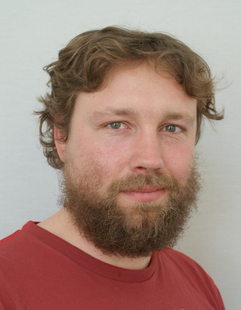
\includegraphics[width=0.2\textwidth]{julian.png}
% \end{wrapfigure}

\MyName{Julian Sagebiel}
\MySlogan{\vspace{-0.3in}\begin{flushright}Department of Economics\\Swedish University of Agricultural Sciences, Uppsala \\
\href{mailto:julian.sagebiel@slu.se}{julian.sagebiel@slu.se}\\
\href{https://www.slu.se/en/ew-cv/julian-sagebiel/}{slu.se}
\end{flushright}}

\sepspace
 \NewPart{Overview}{}
 I am researcher at the ``Decision-making and Managerial Behavior'' group at the Department of Economics at the Swedish University of Agricultural Sciences with a focus on discrete choice modeling in non-market valuation and consumer behavior. I am married and have three children (*2013,*2016,*2018).
%%% Personal details
%%% ------------------------------------------------------------
% \NewPart{Personal Details}{}

% \PersonalEntry{Postal Address}{ Technische Universität Berlin EB 4-2, Straße des 17. Juni 145, D-10623 Berlin, EB 4-2 }
% \PersonalEntry{Marital Status}{not married, 1 daughter, 2 sons}
% \PersonalEntry{Date of Birth}{August, 12, 1983}
% \PersonalEntry{Place of Birth}{Berlin}


%%% Work experience
%%% ------------------------------------------------------------
\NewPart{Appointments}{}

% \noindent \textbf{Professor of Physics} \hfill      % Study
% 		\colorbox{White}{%
% 			\parbox{6em}{%
% 			\hfill\color{Black}2016-$\qquad$}} \par

\EducationEntry{Researcher}{2020-\textcolor{white}{0000}}{Swedish University of Agricultural Sciences}
{\begin{itemize}
\item{Decision making of farmers and consumers}
\item{Economic Experiments (e.g. public good games) and Discrete Choice Experiments}
\item{Teaching: Lectures on Experimental Methods and Statistical Design}
\end{itemize}}
\sepspace

\EducationEntry{Lecturer}{2017-2020}{Technische Universität Berlin}
{\begin{itemize}
\item{Environmental Economics and Consumer Behavior}
\item{Microeconometrics and Discrete Choice Modeling}
\item{Teaching: Courses for Master and Bachelor Students in Environmental Economics and Statistics}
\end{itemize}}
\sepspace

\EducationEntry{Researcher}{2013-2017}{Institute for Ecological Economy Research Berlin}{\begin{itemize}\item{Transdisciplinary Research in Land and Water Management} \item{Empirical Research to Value Non-Market Goods} \item{Survey Design and Analysis}\end{itemize}}
\sepspace
\EducationEntry{Researcher}{2009-2013}{Humboldt-Universität zu Berlin}
{\begin{itemize}\item{Research on Sustainable Megacities} \item {Non-Market Valuation in the Energy Sector in Developing Countries} \item{Applied Work on the Energy Water Nexus in Indian Agriculture}\end{itemize}}


\sepspace
%%% Education
%%% ------------------------------------------------------------
\NewPart{Education}{}

\EducationEntry{PhD Agricultural Economics}{2011-2017}{Humboldt-Universität zu Berlin}{\href{https://edoc.hu-berlin.de/handle/18452/18406?locale-attribute=en}{``Valuing improvements in electricity supply using discrete choice experiments''}\\
Magna Cum Laude. Thesis Advisor: Markus Hanisch}
\sepspace

\EducationEntry{Diploma in Economics}{2003-2008}{Otto-von-Guericke-Universtität Magdeburg}{Title of Thesis: ``Motivstruktur des Altruismus unter Effizienzbedingung''}{Grade 1.8 (good). Research Advisor: Joachim Weimann}



%\newpage


\NewPart{Research Projects}{}

\begin{etaremune}

\item\FundingEntry {Swedish research council for sustainable development (FORMAS)}{\href{https://www.slu.se/en/departments/soil-environment/research/agricultural-water-management-/extreme-weather-and-resilience-in-swedish-agriculture/}{Extreme weather: Risks and solutions to increase the resilience of the Swedish agricultural production}}{Researcher}{2020-2022}

\item\FundingEntry {European Union Horizon 2020}{\href{www.project-contracts20.eu}{Contracts2.0 Innovative contracts for farmers and nature}}{Researcher}{2019-2023}

\item\FundingEntry {German Ministry for Education and Research}{\href{https://www.ioew.de/en/project-single/pado_processes_and_implications_of_dune_breaching_at_the_german_baltic_sea_coast/}{PADO Processes and Implications of Dune Breaching at the German Baltic Sea Coast}}{Researcher}{2016-2018}

\item\FundingEntry {German Ministry for Education and Research}{\href{https://www.ioew.de/en/project-single/value_of_green_urban_spaces/}{Value of Green Urban Spaces Evaluation, Management and Communication as a key for climate resilient and near-natural green spaces}}{Researcher}{2016-2018}


\item\FundingEntry {German Ministry for Education and Research}{\href{https://www.ioew.de/en/project-single/innovative_system_solutions_for_a_transdisciplinary_and_regional_ecological_flood_risk_management_an/}{In\_StröHmunG Innovative System Solutions for a Transdisciplinary and Regional Ecological Flood Risk Management and River Basin Management/Water(course) Development Close to Nature}}{Researcher}{2015-2018}

\item\FundingEntry {German Ministry for Education and Research}{\href{https://secos.deutsche-kuestenforschung.de/}{SECOS The Services of Sediments in German Coastal Seas}}{Researcher}{2013-2016}

\item\FundingEntry {German Ministry for Education and Research}{\href{https://www.cc-landstrad.de/en/}{CC-LandStraD Climate Change – Land Use Strategies in Germany}}{Researcher}{2010-2016}

\item\FundingEntry {German Ministry for Education and Research}{\href{http://www.klimzug-radost.de/en/info}{RA:dOst Regional Adaptation Strategies for the the German Baltic Sea Coast}}{Researcher}{2009-2014}

\item\FundingEntry {DZ Bank Foundation}{\href{https://www.agrar.hu-berlin.de/de/institut/departments/daoe/koopwiss/forschung/energeno}{ENERGENO - Is Electricity from Cooperatives Worth More?}}{Researcher}{2012-2015}

\item\FundingEntry {European Commission}{\href{https://ec.europa.eu/agriculture/external-studies/support-farmers-coop_en}{Support for Farmers’ Cooperatives}}{Consultant}{2011-2012}

\item\FundingEntry {German Ministry for Education and Research}{\href{https://www.iaaw.hu-berlin.de/de/hip/institutes/resecon}{Sustainable Hyderabad: Climate and Energy in a Complex Transition Process towards Sustainability in Hyderabad - Mitigation and Adaptation Strategies by Changing Institutions, Governance Structures, Lifestyles and Consumption Patterns}}{Researcher}{2008-2013}

\end{etaremune}




% \NewPart{Seminars and Colloquia}{}
% \begin{etaremune}
% \item\TalkEntry{Assistant Secretary of Defense for Research \& Engineering}{Basic Research Forum}{4/21/16}{}

% \item\TalkEntry{Rensselaer Polytechnic Institute}{Physics colloquium}{9/24/03}{}
% \end{etaremune}
\NewPart{Teaching}{}

\begin{etaremune}
\item[]
\vspace{-24pt}

\CourseEntry{Winter Term 2020}{Lecture: Experimental methods for economics and business studies}{Swedish University of Agricultural Sciences, Uppsala}

\CourseEntry{2017 to 2020}{Various single lectures within the course Landscape Economics II}{Technische Universität Berlin}

\CourseEntry{Summer Term 2020}{Course: Experiments to Support Decision Making in Environmental Planning part II}{Technische Universität Berlin}

\CourseEntry{Winter Term 2019/20}{Course: Experiments to Support Decision Making in Environmental Planning part I}{Technische Universität Berlin}

\CourseEntry{Summer Term 2019}{Course: Ecosystem Services in Wetlands}{Technische Universität Berlin}

\CourseEntry{Winter Term 2018/19}{Course: Rethinking Urban Space: The Demand for Green Infrastructure}{Technische Universität Berlin}

\CourseEntry{October 2018}{Autumn School: Infrastructure Research and Policy Training (InfraTrain) -- Methodical Track Discrete Choice Experiments}{German Institute for Economic Research (DIW), Berlin}

\CourseEntry{Summer Term 2018}{Course: Applied Statistical Methods in Landscape Planning}{Technische Universität Berlin}

\CourseEntry{Winter Term 2017/18}{Course: The Recreational Value of Urban Green}{Technische Universität Berlin}

\CourseEntry{September 2017}{Summer School: Using Discrete Choice Experiments for the Economic Valuation of Ecosystem Services in Rural Landscapes}{Leibniz Centre for Agricultural Landscape Research}

\CourseEntry{March 2017}{Workshop: Methods for Cooperative Sciences -- Methodical Track Discrete Choice Experiments}{Humboldt-Universität zu Berlin}


\CourseEntry{Summer Term 2015}{Seminar: Economic Valuation of Environmental Goods – Survey Based Methods and Theory}{Humboldt-Universität zu Berlin}

\CourseEntry{February 2015}{Doctoral Seminar Quantitative Methods}{International School of Management, Dortmund}

\CourseEntry{January 2014}{Seminar: Discrete Choice Experiments – Theory and Application}{International School of Management, Dortmund}
\end{etaremune}

\NewPart{Theses Supervised}{}
\begin{etaremune}

\item \ThesisEntry{Marc Ringborg}{2021}{Bachelor Thesis}{Status quo effects of information treatments in discrete choice experiments}{Swedish University of Agricultural Sciences}

\item \ThesisEntry{Giovanni Slinn}{2021}{Master Thesis}{A discrete choice experiment on consumer preferences for tofu characteristics in Germany, Italy, and Sweden}{Swedish University of Agricultural Sciences}

\item \ThesisEntry{Erik Furth}{2021}{Master Thesis}{Floodplain management through economic valuation:Using farmers' preferences to improve pollution-reduction schemes in Germany}{Technische Universität Berlin}

\item \ThesisEntry{Polina Korneeva}{2021}{Master Thesis}{Valuation of carbon sequestration and storage under different land-use management scenarios: A case study in the regiopolis region of Rostock}{Technische Universität Berlin}

\item \ThesisEntry{Ronja Schönau}{2021}{Master Thesis}{Assessing preferences for bicycle infrastructure –
A discrete choice experiment in Seoul, South Korea}{Technische Universität Berlin}

\item \ThesisEntry{Dan Xing}{2020}{Master Thesis}{Discrete choice experiments to measure the economic value of urban green }{Technische Universität Berlin}

\item \ThesisEntry{Ameneh Larijani}{2020}{Master Thesis}{More than a cycle track? New bicycle facility as a measure to improve living quality in Berlin}{Technische Universität Berlin}

\item \ThesisEntry{Luisa Rau}{2020}{Master Thesis}{Is money enough to increase social acceptance of hydropower projects in Southern Chile?}{Technische Universität Berlin}

\item \ThesisEntry{Marisa Ramos Rocha}{2020}{Master Thesis}{Understanding the use of knowledge in decision-making processes to implement nature-based solutions}{Technische Universität Berlin}

\item \ThesisEntry{Jessica Weir and Daniel Soto}{2020}{Master Thesis}{Willingness to pay for sustainable tourism}{Technische Universität Berlin}

\item \ThesisEntry{Bradyn Winiarski}{2020}{Master Thesis}{How Valid is Valid Enough? A Review on Validity of Contingent Valuation for Damage Assessments}{Technische Universität Berlin}

\item \ThesisEntry{Yuhan Miao}{2019}{Master Thesis}{Stated Preferences on the Value of Urban Green Spaces in Germany: How Does the Survey's Consequentiality Influence the Willingness-To-Pay?}{Technische Universität Berlin}

\item \ThesisEntry{Luisa Rau}{2018}{Bachelor Thesis}{The Willingness to Work in Urban Community Gardens as Basis for Political Decision Making: A Contingent Valuation}{Technische Universität Berlin}

\item \ThesisEntry{Katarzyna Malinowska}{2018}{Master Thesis}{The Future of Energy Cooperatives in Germany: Exploring strategic alliances with commercial energy companies}{Humboldt-Universität zu Berlin}

\item \ThesisEntry{Sarah Vitone and Joe Marshall}{2018}{Master Thesis}{The Value of Urban Gardens}{Technische Universität Berlin}

\item \ThesisEntry{Snigdha Sunil Kunder}{2018}{Master Thesis}{Assessing the economic value of the conservation of common toads using a willingness to pay survey}{Technische Universität Berlin}

\item \ThesisEntry{Maria Lindow}{2016}{Master Thesis}{The Role of Cultural Ecosystem Services for the Acceptence of the Local Population with Respect to the Water Framework Directive}{Ernst Moritz Arndt Universität Greifswald}

\item \ThesisEntry{Amely Gundlach}{2016}{Master Thesis}{Overcoming the Tenant Landlord Dilemma:
An Investigation of the Impact of Cooperative Ownership on the Capitalization of Energy Efficiency}{Humboldt-Universität zu Berlin}


\end{etaremune}

\NewPart{Memberships}{}

\begin{itemize}

\item{\href{https://www.agrar.hu-berlin.de/de/institut/departments/daoe/koopwiss/ifg/Institut/vorstand_mitglieder}{Board Member at the \textbf{Institute for Cooperatives at Humboldt-Universität zu Berlin}}} (since 2020)

\item Member of \href{http://www.envecho.com/index.html}{the \textbf{Scientific Network of Researchers using Discrete Choice Modelling in the field of environmental valuation ENVECHO}} (since 2017) 

\item Member of the \href{https://sites.google.com/view/reecap}{\textbf{Research Network on Economic Experiments for the Common Agricultural Policy REECAP}} (Since 2016)

\item Member of {\href{https://www.eaere.org/}{ the \textbf{European Association of Environmental and Resource Economists EAERE}}} (since 2016)

\item Member of {\href{https://eaae.org/}{the \textbf{European Association of Agricultural Economists EAAE}}} (since 2014)

\item Founding Member and Spokesman of the {\href{http://forschungsnetzwerk-energiegenossenschaften.de}{\textbf{Research Network Energy Cooperatives}}} (2014-2016)

\end{itemize}

\NewPart{Further Activities}{}
\begin{itemize}




\item \EducationEntry{\href{http://www.eaere-conferences.org/index.php?y=2021&p=261}{EAERE Conference 2022 Pre-Conference Workshop `Validity of Stated \newline Preference Environmental Valuation using Choice Modelling'}}{2022}{Organizer}{Together with Vic Adamowicz, Klaus Glenk, Robert Johnston and Jürgen Meyerhoff}


\item \EducationEntry{\href{http://fleximeets.com/eaere2020/?p=programme}{EAERE Conference 2020 Thematic Session on `Consequentiality in Stated Preference – New Insights'}}{2020}{Organizer}{Together with Malte Welling and Ewa Zawojska}

\item 
\EducationEntry{\href{https://link.springer.com/journal/10640/75/2}{Special Issue ``Spatial Dimensions of Stated Preferences''}}{2020}{Guest Editor Environmental and Resource Economics Vol. 75/2}{Together with Klaus Glenk, Robert Johnston and Jürgen Meyerhoff}

\item 
\EducationEntry{\href{http://www.landschaftsoekonomie.tu-berlin.de/menue/berlin_dce_colloquium/}{Berlin Discrete Choice Colloquium}}{Since 2016}{Founding Member and Organizer}{Together with Jürgen Meyerhoff}

\item \EducationEntry{\href{http://communications.ext.zalf.de/sites/dce/SitePages/DCE\%20Summer\%20School.aspx}{Summer School `Using Discrete Choice Experiments for the \newline Economic Valuation of Ecosystem Services in Rural Landscapes'}}{2014-2016}{Organizer and Lecturer}{Together with Kati Haefner, Jürgen Meyerhoff and Jens Rommel}

\item \EducationEntry{\href{http://www.eaere-conferences.org/index.php?p=60}{EAERE Conference 2017 Pre-Conference Workshop `Spatial \newline Dimensions of Stated Preferences'}}{2016-2017}{Organizer}{Together with Klaus Glenk, Robert Johnston and Jürgen Meyerhoff}


\item \EducationEntry{\href{https://eaere2016.ethz.ch/programme/scientific-programme/thematic-sessions.html}{EAERE Conference 2016 Thematic Session on `Willingness to Pay \newline in Space: New Insights into the Spatial Dimensions of Stated \newline Preferences'}}{2016}{Organizer}{Together with Robert Johnston and Jürgen Meyerhoff}

\item \EducationEntry{Occasional scientific consultancies}{Since 2012}{Survey Engine GmbH ($>100$h), International School of Management gGmbH ($>50$h), European Commission ($>40$h), Centre for Rural Development at Humboldt-Universität zu Berlin ($>30$h)}{}


\end{itemize}



 \NewPart{Awards}{}
 \begin{itemize}
 
 
\item 2017 \href{https://www.agrar.hu-berlin.de/de/institut/departments/daoe/koopwiss/ifg/forschung/wissenschaftlicher-nachwuchs/raiffeisen-schulze-delitzsch-foerderpreis}{Raiffeisen - Schulze-Delitzsch-Förderpreis 2016} for the best dissertation in cooperative sciences in 2016
 \item 2017 German Academic Exchange Service (DAAD) Travel Grant for the \textit{Environmental and Resource Economics} Conference in Athens
 \item 2016 German Academic Exchange Service (DAAD) Travel Grant for the \textit{Environmental and Resource Economics} Conference in Zurich
 \item 2007 German Academic Exchange Service (DAAD) Grant for a Study Exchange Semester at \textit{Macquarie University Sydney}, Australia

\end{itemize}

% \NewPart{Major Departmental Committees Chaired}{}
% \begin{itemize}
% \item Graduate qualifier exam committee, 2016-present (manage authorship of both Classical and Quantum exams each semester)
% \item CME faculty search committee, 2013 (hired V. Manucharyan and J. Williams)
% \item Undergraduate curriculum review committee, 2011 (authored 50+ page report)
% \end{itemize}

%\newpage



\NewPart{Software}{}
Stata (Expert), R (Expert), \LaTeX (Expert),  LIMDEP (Advanced), NGENE (Expert), Latent Gold (Advanced), Biogeme (Advanced), Python (Intermediate), Bash (Intermediate), Z-Tree (Intermediate)

\NewPart{Reviewer Activities}{\href{https://publons.com/a/1337890}{[Publons]}}
Ecological Economics (8), Energy Research \& Social Science (5), 
Energy Economics (4), 
Environmental Science and Pollution Research (4), Journal of Environmental Economics and Management 
(2), 
Energy Policy (1),
 Environmental and Resource Economics (1), European Review of Agricultural Economics (1), Journal of Behavioral and Experimental Economics (1), 
 Journal of Environmental Economics and Policy
(1), Land Use Policy
(1), Scientific Reports
(1), Utilities Policy
(1), Water Resources and Economics (1)


%  \NewPart{References}{}
%  \begin{itemize}
% \item Dr. Jürgen Meyerhoff (Technische Universität Berlin)
% \item Prof. Dr. Markus Hanisch (Humboldt-Universität zu Berlin)
%\end{itemize}

\newpage

%%% Papers
%%% ------------------------------------------------------------

\NewPart{Papers under Review}{}{}






 

\begin{etaremune}

\item \bibentry{zawojska2021}

\item \bibentry{villa2021}

\item \bibentry{Rommel2021}

\item \bibentry{Welling2021}

\item \bibentry{Giergiczny2021}

\item \bibentry{rogers2021}


\end{etaremune}


\NewPart{Peer-Reviewed Journal Papers}{\href{https://scholar.google.de/citations?user=RzdZi_IAAAAJ&hl=de}{[citations]}}


\begin{etaremune}
\item \bibentry{sagebiel2020does}
\item \bibentry{sagebiel2020clean}
\item \bibentry{fruth2020discrete}
\item \bibentry{fruth2019economic}
\item \bibentry{villamayor2019bringing}
\item \bibentry{Glenk2019}
\item \bibentry{knoefel2018consumer}
\item \bibentry{gundlach2018investigating}
\item \bibentry{muller2018structural}
\item \bibentry{rayanov2018economic}
\item \bibentry{ghosh2017small}
\item \bibentry{rommel2017preferences}
\item \bibentry{sagebiel_preference_2017}
\item \bibentry{sagebiel_spatially_2017}
\item \bibentry{kimmich_empowering_2016}
\item \bibentry{sagebiel2016economic}
\item \bibentry{rommel_quality_2016}
\item \bibentry{magliocca2015meta}
\item \bibentry{sagebiel_are_2014}
\item \bibentry{sagebiel_preferences_2014}
\item \bibentry{hanisch_coping_2010}



\end{etaremune}



\NewPart{Book Chapters}{}
\begin{etaremune}
\item \bibentry{Elsasser2021}
\item \bibentry{Yildiz2019}
\item \bibentry{sagebielbuilding2014}
\item \bibentry{kimmich_peri-urban_2013}
\item \bibentry{sagebiel_governance_2013}
\item \bibentry{rommel_nachhaltige_2012}
\end{etaremune}


\NewPart{Books}{}
\begin{etaremune}
\item \bibentry{marielenvironmental}
\item \bibentry{sagebiel2017valuing}
\item \bibentry{sagebiel_enhancing_2016}
\item \bibentry{kimmich_methods_2012} 
\end{etaremune}


\newpage
% \bibliographystyle{apalike}
% \bibliography{publ}
\end{document}
